% !TEX TS-program = lualatex
% !TEX encoding = UTF-8 Unicode

% This is a simple template for a LaTeX document using the "article" class.
% See "book", "report", "letter" for other types of document.

\documentclass[10pt, twocolumn]{article} % use larger type; default would be 10pt

\usepackage[utf8]{inputenc} % set input encoding (not needed with XeLaTeX)
\usepackage{fontspec}
\setmainfont{Georgia}
\setsansfont{Georgia}
\setmonofont{Georgia}
%\usepackage[none]{hyphenat}
\usepackage{hyphenat}

%%% Examples of Article customizations
% These packages are optional, depending whether you want the features they provide.
% See the LaTeX Companion or other references for full information.

%%% PAGE DIMENSIONS
\usepackage{geometry} % to change the page dimensions
\geometry{a4paper, left=17.5mm, right=17.5mm, textwidth=85mm,columnsep=5mm, top=17.5mm}
\setlength{\parindent}{0pt}
% or letterpaper (US) or a5paper or....
% \geometry{margin=2in} % for example, change the margins to 2 inches all round
% \geometry{landscape} % set up the page for landscape
%   read geometry.pdf for detailed page layout information

\usepackage{subcaption}
\usepackage{graphicx} % support the \includegraphics command and options

\usepackage[parfill]{parskip} % Activate to begin paragraphs with an empty line rather than an indent

%%% PACKAGES
\usepackage{booktabs} % for much better looking tables
\usepackage{array} % for better arrays (eg matrices) in maths
\usepackage{paralist} % very flexible & customisable lists (eg. enumerate/itemize, etc.)
\usepackage{verbatim} % adds environment for commenting out blocks of text & for better verbatim
%\usepackage{subfig} % make it possible to include more than one captioned figure/table in a single float
\usepackage{amsmath}
% These packages are all incorporated in the memoir class to one degree or another...
\usepackage{lipsum}
%\usepackage{caption}
\usepackage{listings}

%%% HEADERS & FOOTERS
\usepackage{fancyhdr} % This should be set AFTER setting up the page geometry
\pagestyle{fancy} % options: empty , plain , fancy
\renewcommand{\headrulewidth}{0pt} % customise the layout...
\lhead{}\chead{}\rhead{}
\lfoot{}\cfoot{\thepage}\rfoot{}

%%% SECTION TITLE APPEARANCE
%\usepackage{sectsty}
%\allsectionsfont{\sffamily\mdseries\upshape} % (See the fntguide.pdf for font help)
% (This matches ConTeXt defaults)

%%% ToC (table of contents) APPEARANCE
\usepackage[nottoc,notlof,notlot]{tocbibind} % Put the bibliography in the ToC
\usepackage[titles,subfigure]{tocloft} % Alter the style of the Table of Contents
\renewcommand{\cftsecfont}{\rmfamily\mdseries\upshape}
\renewcommand{\cftsecpagefont}{\rmfamily\mdseries\upshape} % No bold!
\usepackage{authblk}

\usepackage{float}

\newcommand{\overbar}[1]{\mkern 1.5mu\overline{\mkern-1.5mu#1\mkern-1.5mu}\mkern 1.5mu}

%%% END Article customizations

%%% The "real" document content comes below...

\title{\textbf{Tunable in twisted bilayer NbSe$_2$}}
\author{Conan Birkett}
\affil{Department of Physics, University of Bath, Bath BA2 7AY, United Kingdom}
%\date{} % Activate to display a given date or no date (if empty),
         % otherwise the current date is printed 

\begin{document}
\twocolumn[
 \begin{@twocolumnfalse}
\maketitle
\begin{abstract}
  Following observation of unconventional superconductive effects in twisted bilayer graphene, the novel field of 'twistronics' has seen a rapid progression in theory and experiment. When a Van der Vaals heterostructure formed from a bilayer of 2D lattices is twisted at a so-called 'magic-angle' perturbation effects and interlayer tunneling lead to the formation of a flat electronic band at fermi level in some materials. These exotic electronic properties have the potential to be exploited as high temperature superconductors or in novel electronic devices. Using a multiorbital tight binding model (TBM) we model a bilayer of transition metal dichalcogenide 2H-NbSe$_2$ with interlayer tunneling at various twist angles. We observe ***** in the electronic band structure at *** points. Our results show potential for further modelling of the NbSe$_2$.

\bigskip
\end{abstract}
\end{@twocolumnfalse}
]
\medskip

\section*{Introduction}

  In 2018 Cao Y. et al\cite{Cao2018} realised unconventional superconductivity in bilayer graphene twisted to the 'magic-angle' of 1.1$^\circ$ 

\section*{Method}
  Our work draws on several published methods on NbSe2 and twistronics. In particular we take the multiorbital tight binding model of monolayer NbSe2 from Habara and Wakabayashi\cite{Habara2021}. To model the bilayer with twist, we employ the method used in the original magic-angle paper by Bistritzer and MacDonald \cite{Bistritzer2011}. 

\subsection*{Monolayer NbSe2}
  NbSe$_2$ is a two dimensional (2D) transition metal dichalcogenide (TMDC) specifically it is a group-V TMDC with formula $MX_2$ for $M =$ Nb, Ta and $X =$ S, Se. It has metallic properties with superconductivity at temperatures near ~ $X$ K. It also exhibits a strong spin orbit coupling (SOC) field which results in Ising-type spin orbit coupling, i.e. strong effective Zeeman field that holds electron spins in out-of-plane directions. We employ a multiorbital tight binding model (TBM) of NbSe2 as described by Habara and Wakabayashi \cite{Habara2021}. We take a basis of $d_{z^2}$, $d_{x^2 - y^2}$ and $d_{xy}$ orbitals of the Nb atoms with spin orbit coupling. These states are dominant in the electronic band near fermi level. We take this as an adequate description of the NbSe$_2$ monolayer for low energy electronic states.

\begin{figure}[t]
\centering
  \begin{subfigure}[t]{0.45\textwidth}
    \centering
    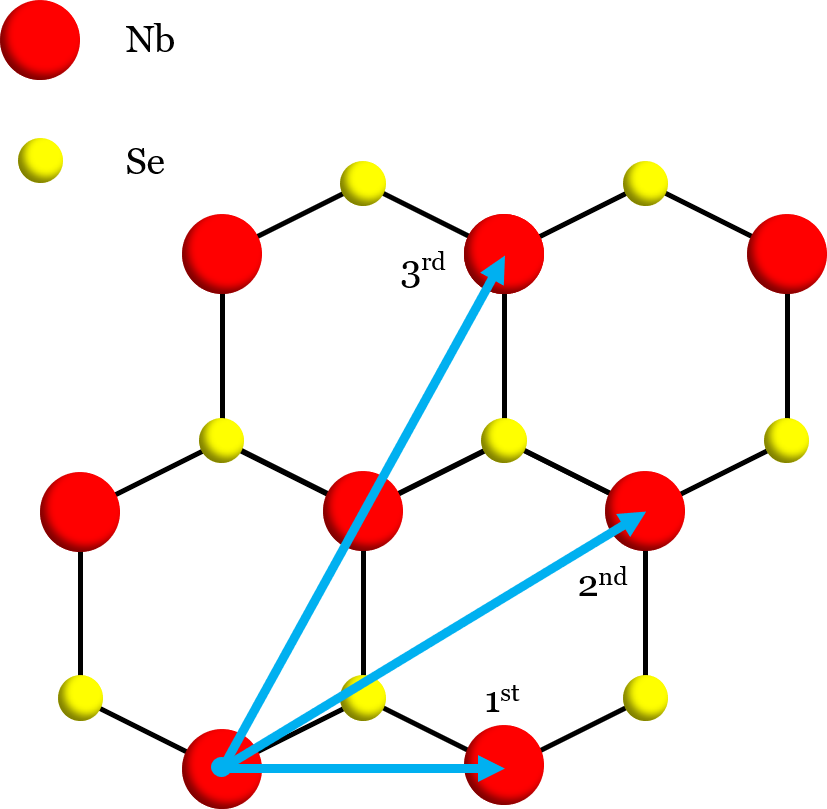
\includegraphics[width=0.95\textwidth]{NbSe_top.png}
    \caption{
      Top view of NbSe$_2$ with example nearest neighbours (NN) up to third NN sites.
    }
  \end{subfigure}
  \hfill
  \begin{subfigure}[t]{0.45\textwidth}
    \centering
    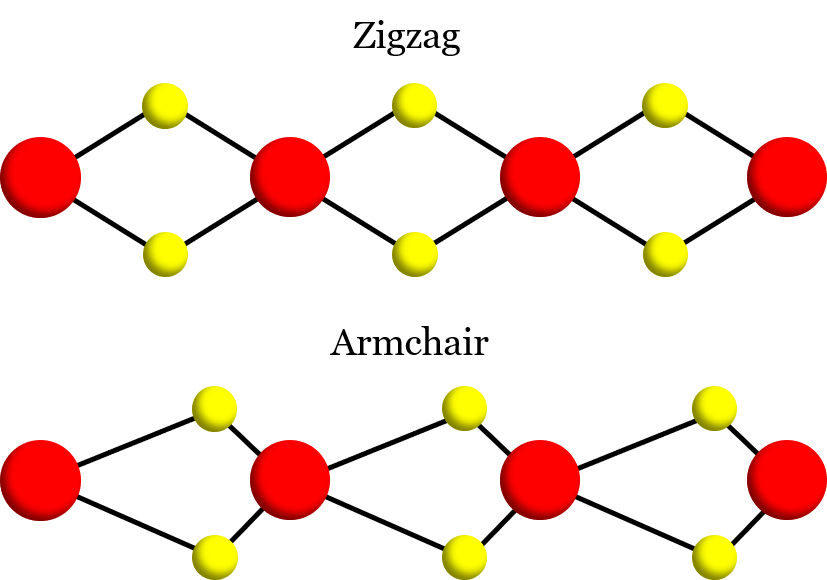
\includegraphics[width=0.95\textwidth]{NbSe_side.png}
    \caption{
      Side view of NbSe$_2$ from the 'zigzag' edge, Se atoms are directly above and below each other in out-of-plane axis.
    }
  \end{subfigure}
  \caption{
    Monolayer NbSe$_2$
  }
\end{figure}

\begin{figure}[t!]
\centering
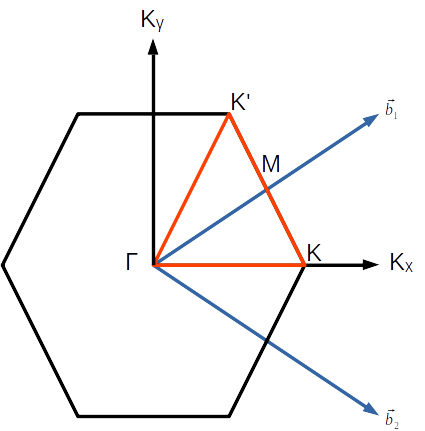
\includegraphics[width=0.95\columnwidth]{1st_BZ.png}
  \caption{
    First Brilloin zone in a hexagonal lattice. shown are: reciprocal lattice vectors $b_1, b_2$, standard critical points $\Gamma, K, K', M$ and wavevector axes $k_x, k_y$. Electronic bands are found for $k$ sampled from the equilateral triangle $\Gamma \rightarrow K \rightarrow M \rightarrow K' \rightarrow \Gamma$ or $\Gamma \rightarrow \Gamma$ shown in red.
  }
  \label{1st_BZ_diagram}
\end{figure}

  The TBM considers the interactions of these electronic states up to the third nearest neighbour sites.

  The eigenvalue equation of the TBM is 
      \begin{equation}
        \label{TBM_evalue_eqn}
        \hat{H}(k)\left|u_{n k}\right\rangle=E_{n k}\left|u_{n k}\right\rangle,
      \end{equation}

   where $k=\left(k_{x}, k_{y}\right)$ is the wave-number vector, $E_{nk}$ is the eigenvalue and $n = 1,2,\cdots,6$ is the band index.

   we define the eigenvector as
      \begin{equation}
        \begin{aligned}
          |u_{n k}\rangle=( & c_{n k, d_{z^{2}}, \uparrow}, c_{n k, d_{x y}, \uparrow}, c_{n k, d_{x^{2}-y^{2}}, \uparrow},\\
          & c_{n k, d_{z^{2}}, \downarrow}, c_{n k, d_{x y}, \downarrow}, c_{n k, d_{x^{2}-y^{2}}, \downarrow})^{T}
        \end{aligned}
      \end{equation}

  where $(\cdots)^T$ indicates the transpose of the vector and $c_{nk\tau s}$ is the amplitude at atomic orbital $\tau$ with spin $s$ for the $n$th energy band at $k$.

  The monolayer hamiltonian $\hat{H}(k)$ with spin orbit coupling is then 
      \begin{equation}
        \hat{H}(k)=\hat{\sigma}_{0} \otimes \hat{H}_{\mathrm{TNN}}(k)+\hat{\sigma}_{z} \otimes \frac{1}{2} \lambda_{\mathrm{SOC}} \hat{L}_{z}
      \end{equation}

  with the TBM nearest neighbour hamiltonian

      \begin{equation}
        \hat{H}_{\mathrm{TNN}}(k)=\left(\begin{array}{ccc}
        V_{0} & V_{1} & V_{2} \\
        V_{1}^{*} & V_{11} & V_{12} \\
        V_{2}^{*} & V_{12}^{*} & V_{22}
        \end{array}\right)
      \end{equation}

  and spin orbit coupling term

      \begin{equation}
        \hat{L}_{z}=\left(\begin{array}{ccc}
        0 & 0 & 0 \\
        0 & 0 & -2 i \\
        0 & 2 i & 0
        \end{array}\right)
      \end{equation}

  $\hat{\sigma}_0$ and $\hat{\sigma}_z$ are pauli matrices and $\lambda_{\text{SOC}}=0.0784$ eV is the Ising-type spin orbit coupling parameter. The potentials $V_0 \cdots V_{22}$ in the TNN hamiltonian are functions of $k$ determined from the nearest neighbour hopping vectors with fitting parameters.

  The resulting monolayer hamiltonian $\hat{H}(k)$ is a 6x6 block diagonal hermitian matrix as a function of wavevector $k$. The eigenvalues of this hamiltonian correspond to the energy of the 6 eigenstates / electronic bands for a given point in reciprocal space $k$. When determining the electronic bands, we take $k$ from slices in the first brilloin zone along the standard critical points: $\Gamma, K, K', M$. By Bloch's theorem we can describe the electronic properties of the whole monolayer by considering the region bounded by these points due to the periodicity of potentials in the lattice and reflectional symmetry. Specifically, $k$ bounded by the equilateral triangle $\Gamma \rightarrow K \rightarrow M \rightarrow K' \rightarrow \Gamma$, hereafter refered to as $\Gamma \rightarrow \Gamma$.

\subsection*{Modelling a twist}

  Before constructing a twisted bilayer we first consider a monolayer twisted by some angle $theta$. A rotation in primitive lattice vectors $a_1, a_2 \rightarrow a_1', a_2'$ corresponds to the same rotation in reciprocal lattice vectors $b_1, b_2 \rightarrow b_1', b_2'$. We can treat this rotation as a rotation of the coordinate system in $k$ space: $(k_x, k_y) \rightarrow (k_x', k_y')$. Then, for some vector $k' \in (k_x', k_y')$ we can find the same vector $k'$ in our original wavevector basis $(k_x, k_y)$ by rotating it by $-\theta$.

\begin{figure*}[t]
\centering
  \begin{subfigure}[t]{0.45\textwidth}
    \centering
    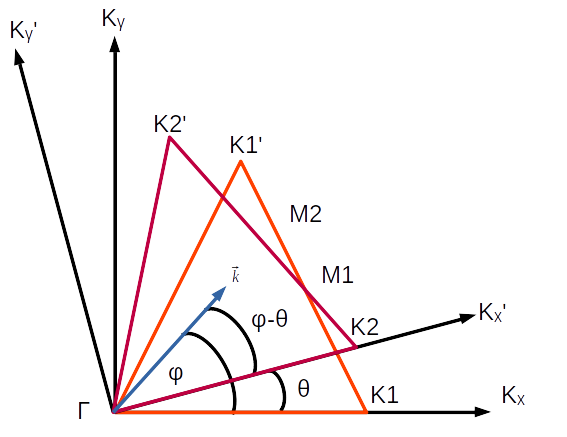
\includegraphics[width=0.95\textwidth]{twisted_triangles.png}
    \caption{
      Equilateral triangle from first Brilloin zone shown in unrotated and relatively rotated (by angle $\theta$) reciprocal coordinate systems. An arbitrary vector $k$ in the rotated basis $(k_x', k_y')$ must first be rotated by $-\theta$ before it can be projected onto the unrotated basis $(k_x, k_y)$
    }
  \end{subfigure}
  \hfill
  \begin{subfigure}[t]{0.45\textwidth}
    \centering
    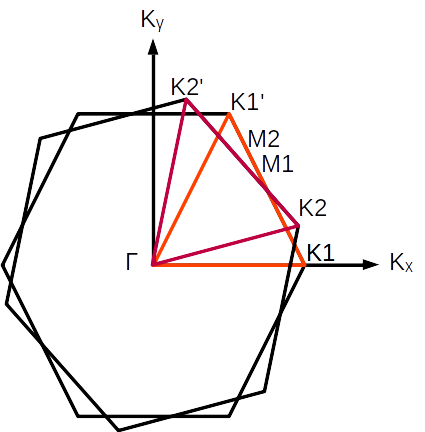
\includegraphics[width=0.95\textwidth]{heterostructure_BZ_path.png}
    \caption{
      Brilloin zones of both layers at relative angle $\theta$ overlayed. Evaluation of the electronic bands is taken on the set $\Gamma \rightarrow K1 \rightarrow M1 \rightarrow K1' \rightarrow \Gamma \rightarrow K2 \rightarrow M2 \rightarrow K2' \rightarrow \Gamma$ or $\Gamma \rightarrow \Gamma \rightarrow \Gamma$.
    }
  \end{subfigure}
  \caption{
  }
\end{figure*}

  If we consider the equilateral triangle in reciprocal space $\Gamma \rightarrow K1 \rightarrow M1 \rightarrow K1' \rightarrow \Gamma$ taken on an unrotated basis. We can construct a rotated triangle $\Gamma \rightarrow K2 \rightarrow M2 \rightarrow K2' \rightarrow \Gamma$. For the the evaluation of electronic bands in a twisted bilayer we sample $k$ from the path $\Gamma \rightarrow K1 \rightarrow M1 \rightarrow K1' \rightarrow \Gamma \rightarrow K2 \rightarrow M2 \rightarrow K2' \rightarrow \Gamma$ or in shorthand $\Gamma \rightarrow \Gamma \rightarrow \Gamma$

\subsection*{Twisted bilayer}

  NbSe$_2$ monolayers are held together by a weak Van-der-Waals interaction, this allows for the stacking of multiple layers - specifically a bilayer. Because of the weak bonding it is possible to orient these layers at twist angles relative to each other. Through this rotation and by inter-layer tunneling we aim to explore novel electronic properties in twisted bilayers.

  To describe the electronic states in a twisted bilayer we can initially start with a simple model with no interaction between states in different layers. We construct the hamiltonian of the whole system by taking a block diagonal hamiltonian matrix $\hat{H}{k}$ from two monolayer matrices $\hat{H_1}{k}$ and $\hat{H_2}{k'}$
%
      \begin{equation}
        \hat{H}(\boldsymbol{k})=\left(\begin{array}{cc}
          \hat{H_1}(\boldsymbol{k}) & 0\\
          0 & \hat{H_2}(\boldsymbol{k'})
        \end{array}\right)
      \end{equation}
      
  where $\hat{H_2}(k')$ is the Hamiltonian of the second monolayer, which is rotated by angle $\theta$ relative to the first. To find $\hat{H}(k)$ we must rotate $k$ to $k'$ (as described previously) in $\hat{H_2}(k')$.

  continuing, we will denote rotated vectors as $v'$ where the rotation is relative to a vector on the 'unrotated layer' $v$. We will also denote these layers by index, layer 1 is unrotated, layer 2 is rotated relative to layer 1.

\subsection*{Interlayer tunneling}
  To model inter-layer electron tunneling we follow the method of Bistritzer and MacDonald \cite{Bistritzer2011} for graphene, which is outlined for a more general case by Koshino \cite{Koshino2015}.

  For reciprocal lattice vectors $b_i, b_i'$ where $b_i'$ is the equivalent reciprocal lattice vector of the rotated layer. We can show that
  \begin{equation}
    k + G = k' + G',
    \label{inter-layer_k_plus_G}
  \end{equation}
  where $G = m_1 b_1 + m_2 b_2 \text{ and } G' = m_1 b_1' + m_2 b_2'$ are reciprocal lattice vectors of the unrotated and rotated layers respectively.

  This is because a bloch state on layer 1 $\phi_k^{(1)}$ is a summation of $e^{i(k+b)}$ over reciprocal vectors. Similarily, on layer two $\phi_{k'}^{(2)}$ is a sum over $e^{i(k'+b')}$. The system hamiltonian is described by fourier components of $G, G'$. So the matrix element $\langle \phi_{k'}^{(2)} | \hat{H} | \phi_{k}^{(1)}$ is only non-zero if \ref{k_plus_b} holds. The derivation of \ref{k_plus_b} is as follows:

  First we assume that equivalent unit cells in both layers $X$ and $X'$ have multiple atomic orbitals with real space lattice positions
  \begin{equation}
    \begin{gathered}
    R_X = n_1 a_1 + n_2 a_2 + \tau_X,\\
    R_{X'} = n_1 a_1' + n_2 a_2' + \tau_{X'},
    \end{gathered}
    \label{inter-layer_real_sublattice_positions}
  \end{equation}

  for $n_1, n_2 \in \mathrm{N}$ and primitive lattice vectors $a_1, a_2$ and $a_1', a_2'$ in either respectively. $\tau_X$ are the sublattice positions of the atomic states in unit cell $X$

  We define $| R_x \rangle \equiv \phi(r - R_X)$ is the atomic state of sublattice $X$ at localised in real position $R_X$

  The interlayer hamiltonian elements are then
  \begin{equation}
    U = -\sum_{X, X'} T_{X'X}(R_{x'} - R_x) |R_{x'}\rangle \langle R_x|,
    \label{inter-layer_hamiltonian_elements}
  \end{equation}

  where the inter-layer transfer potential $-T_{X'X}(R_{x'} - R_x)$ is a function of the real space positions of the atomic orbitals, the specifics of this function we shall discuss later.

  We define the Bloch basis in each layer as the summation over unit cells (and thus primitive lattice vectors)
  \begin{equation}
    | k,j,l \rangle = \frac{1}{\sqrt{N_l}}\sum_{R_X}e^{ik\cdot(R+\tau_i)}\phi_j(r-R-\tau_j, z-z_l)
    \label{inter-layer_real_bloch_basis}
  \end{equation}

  for wavevector $k$, sublattice $j$ and layer index $l$ where $N_l$ is the number of unit cells in layer $l$. $\phi_j (r - R - \tau_j, z-z_l)$ is the wavefunction in 2d real space in the plane and out of plane.

  Our inter-layer hopping Hamiltonian elements are then given by
  \begin{multline}
    \langle k',j',l' | U | k, j, l \rangle = \\
    ~\\
    \frac{1}{\sqrt{N_l N_{l'}}} \sum_{R, R'} e^{ik \cdot (R+\tau_j)} e^{-ik' \cdot (R' + \tau_{j'})} \times \\
    \langle \phi_{j'}(r - R' - \tau_{j'}, z - z_{l'}) | U | \phi_j (r - R - \tau_j, z - z_l)\\
    ~\\
     =\frac{1}{\sqrt{N_l N_{l'}}} \sum_{R, R'} e^{ik \cdot (R+\tau_j)} e^{-ik' \cdot (R' + \tau_{j'})} \times \\
     t(R'-R +\tau_{j'} - \tau_j, z_l' - z_l),
    \label{}
  \end{multline}

  where we invoke a two centre approximation, the hopping between sites is a function of their distance only. We also assume that the the hopping $t(\vec{r_{2D}}, z)$ does not depend on the direction of $\vec{r_{2D}}$ i.e. $t(\vec{r_{2D}}, z) = t(|\vec{r_{2D}}|, z)$

  For a large superlattice period, the relative inter atomic positions for every combination of atomic sites are required. It is easier to reconstruct the hamiltonian in reciprocal space.

  By taking a fourier transform (see appendix) we can show that
  \begin{equation}
    \langle k',j',l' | U | k, j, l \rangle = \sum_{G, G'} t(k'+G', z) \delta_{k-G, k'+G'},
    \label{inter-layer_hopping_elements}
  \end{equation}
  
  which yields the result in \ref{inter-layer_k_plus_G}
  
  As we are taking the interlayer tunneling to be a function of $k+G$ we only consider $G, G'$ of magnitude $\leq$ the reciprocal lattice constant $b$. The result is that for a given $k, k'$ we have seven pairs of permissible $G, G'$ that obey \ref{inter-layer_k_plus_G} we define them as follows: $G_0$ is the zero vector, $G_1, G_2$ are equal to reciprocal lattice vectors $b_1, b_2$, $G_{3,\cdots,4}$ continue from reciprocal lattice vectors in a clockwise fashion.

  We define
  \begin{equation}
    G_i^M = G_i - G_i'
    \label{inter-layer_G_M_def}
  \end{equation}
  such that \ref{inter-layer_k_plus_G} becomes
  \begin{equation}
    k' = k + G^M
    \label{inter-layer_k_plus_G_M}
  \end{equation}

  So for a given point on layer one $k_0$, we have a well defined set of seven permissible $k'$ points on the layer two that tunneling is allowed between.

\begin{figure}[t!]
\centering
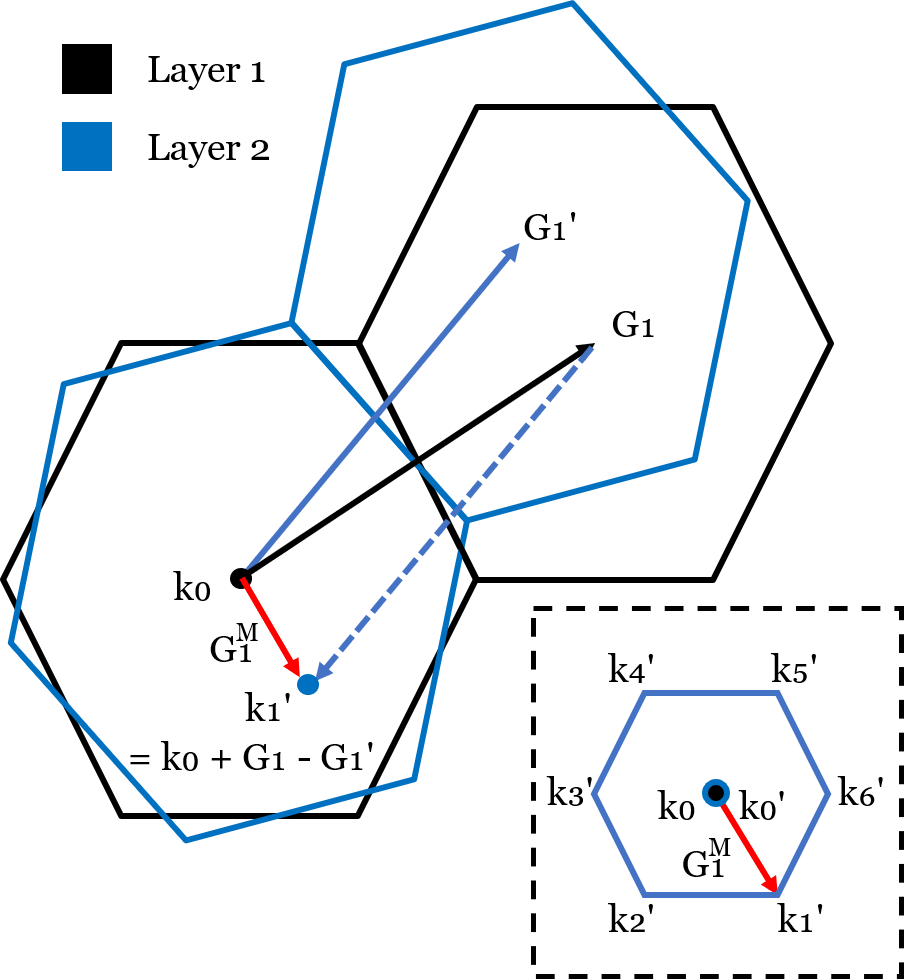
\includegraphics[width=0.95\columnwidth]{k_prime_diagram.png}
  \caption{
  }
  \label{inter-layer_k_prime_diagram}
\end{figure}



  Previously our Hamiltonian was a $12\times12$ function of $k$. Now, with the  addition of inter-layer tunneling we have an $84\times84$ Hamiltonian with interlayer tunneling potential on the off-diagonal blocks.

\subsection*{Tunneling potential}

The tunneling potential $t(k + G, z)$ we model as a gaussian in the in-plane axes and assume $z$ constant
\begin{equation}
  t(k + G) = \frac{C\pi}{A_{UC} r_0^2}e^{- r_0^2 (k + G)/4}
\end{equation}

\subsection*{Implementation}

\section*{Results and discussion}

\subsection*{Monolayer electronic bands}

\begin{figure}[t!]
\centering
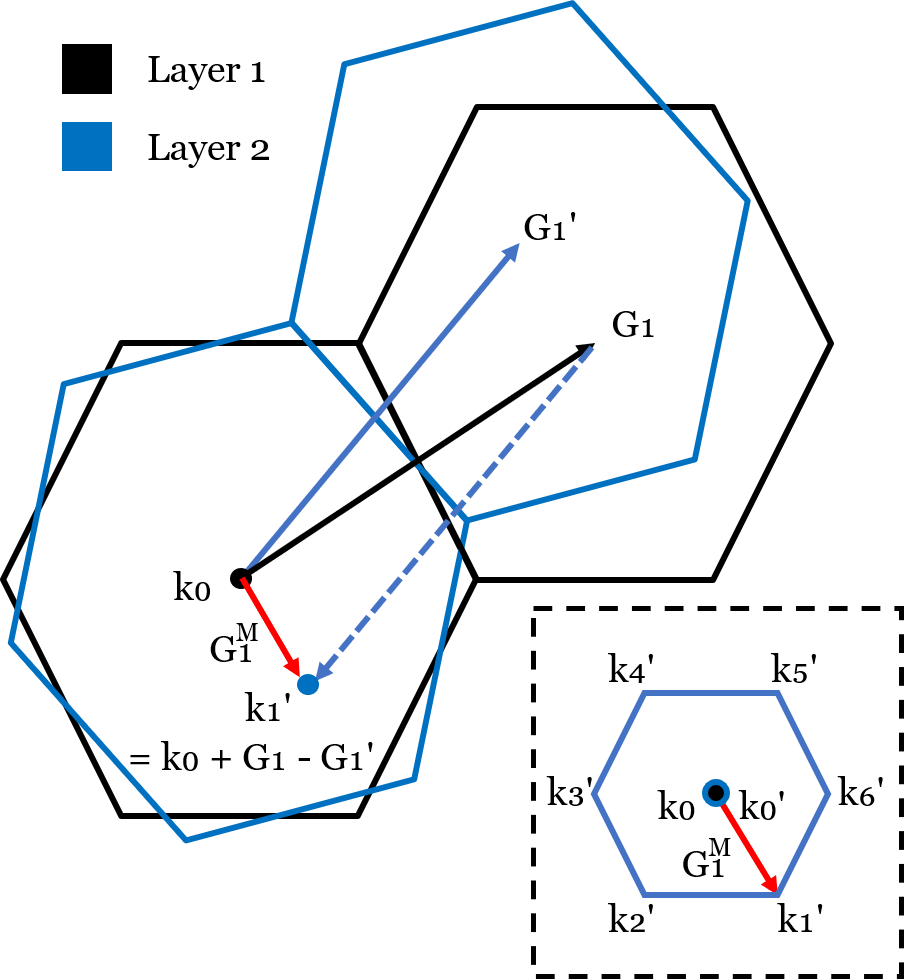
\includegraphics[width=0.95\columnwidth]{k_prime_diagram.png}
  \caption{
  }
  \label{inter-layer_k_prime_diagram}
\end{figure}

\subsection*{Bilayer electronic bands}

\subsection*{Inter-layer tunneling}

\section*{Conclusion}


\section*{Acknowledgements}
I would like to acknowledge the contributions of my project partner Sanjana Reddy and my project supervisor Dr Marcin Mucha-Kruczynski.

%%%References
\bibliographystyle{ieeetr}
%bibliographystyle{bathx}
\bibliography{refs}

\clearpage

\onecolumn

\section*{Appendix}

\subsection*{Inter-layer tunneling Hamiltonian derivation}

\subsection*{Implementation of algorithm}
  The DLA data discussed in this report was generated by an implementation of the described DLA algorithm in C++. Standard C++ libraries are used for sampling of 'true' and psuedo-random numbers used in the random walk and particle generation. Utilities were written to record multiple simulations with varying parameters and to export recorded data from simulations to a csv format. Data analysis and derivation of fractal dimension was performed in Python using the numpy and pandas libraries. All computations were performed on a 64-bit desktop processor running Linux Mint 20.1 'Ulyssa'.

  \textbf{Note: when compiling and running the C++ code provided, the makefile in 'source' has been edited. To compile the code place the .cpp and .h files into a directory called 'source' and add in the missing/unedited files (Particle.h, Window.h, Window.cpp). Run 'make -B -C ./source/' from the directory above 'source'. The compiled binary and the data it produces are in this directory, execute the binary using './run'. The python data analysis file 'DLA.py' should also be run from this same directory}

  The changes made to the C++ code given by Dr A. Souslov and Dr D. Tsang are spread throughout the source code provided (i.e: CSVWrite.h, DLASystem.cpp, DLASystem.h, mainDLA.cpp, rnd.h, Makefile). Most of the changes made are used when pressing 't' in the simulation window to set parameters for data recording and $P_{stick}$ etc. Some new functions have been added to the DLASystem class, and a new class CSVWrite is written for data recording. Some select functions are presented here but you would do best to look at the source code with comments.

\begin{lstlisting}
//write recorded data to a CSV file
void DLASystem::writeDataCSV(){
  auto csv = new CSVWrite("./data.csv");

  csv->WriteVector(dataSet);
  csv->CSVClose();

  //clearDataSet();

  recording = false; //should be false anyways
}
\end{lstlisting}

\end{document}
